\documentclass[12pt,a4paper]{report}
\setlength\textwidth{145mm}
\setlength\textheight{247mm}
\setlength\oddsidemargin{15mm}
\setlength\evensidemargin{15mm}
\setlength\topmargin{0mm}
\setlength\headsep{0mm}
\setlength\headheight{0mm}

\setcounter{secnumdepth}{6}

\usepackage[utf8]{inputenc}
\usepackage{graphicx}
\usepackage{subfig}  
\usepackage{multirow}
\usepackage{float}
\usepackage{datetime}
\usepackage[table,xcdraw]{xcolor}

\usepackage{amsthm}
\usepackage{hyperref}


\renewcommand{\contentsname}{Contenido}
\makeatletter
\def\@makechapterhead#1{
  {
    \parindent \z@ \raggedright \normalfont
    \Huge\bfseries \thechapter. #1
    \par\nobreak
    \vskip 20\p@
  }
}
\def\@makeschapterhead#1{
  {
    \parindent \z@ \raggedright \normalfont
    \Huge\bfseries #1
    \par\nobreak
    \vskip 20\p@
  }
}
\makeatother

\def\chapwithtoc#1{
  \chapter*{#1}
  \addcontentsline{toc}{chapter}{#1}
}

\begin{document}

  \pagestyle{empty}
  \begin{center}

    \large{Universidad Distrital Francisco Jos\'e de Caldas}
    
    \medskip{Facultad de ingeniería}

    \vfill
    {\bf\Large }

    \vfill
    \begin{figure}[h]
      \centering
      \vspace{5mm}	% Adjust vertical spacing here
      
\includegraphics[width=0.7\linewidth]{ima/logoud_0_php7YvUJr}
    \end{figure}

    \vfill
    \vspace{5mm}
    {\large Juan Felipe Rodr\'iguez Galindo}

    \vspace{5mm}
    {\large\bfseries Modelo de un criptosistema esteganogr\'afico a través de audio basado en redes neuronales y atractores ca\'oticos para el cifrado de im\'agenes}

    \vfill
    Bogotá D.C.

    \vfill
    \date{\today}
  \end{center}

  \newpage

  \pagestyle{empty}
  \begin{center}

    \large
    Universidad Distrital Francisco Jos\'e de Caldas
    
    \medskip
    Facultad de ingeniería

    \vfill
    \vspace{5mm}
    {\large Juan Felipe Rodríguez Galindo}

    \vspace{15mm}
    {\large\bfseries Modelo de un criptosistema esteganogr\'afico a través de audio basado en redes neuronales y atractores ca\'oticos para el cifrado de im\'agenes}

    \vfill
    Anteproyecto de grado presentado como requisito parcial para optar al título de Ingeniero de Sistemas

    \vfill
    Directoras: \\
    \vspace{5mm}
    Edilma Isabel Amaya Barrera\\
    Magister en Ciencias Matemáticas\\
    \vspace{3mm}
    Luz Deicy Alvarado Nieto\\
    Doctora en Ciencias de la Computación e Inteligencia Artificial\\
    \vfill
    %Firma:\rule{50mm}{0.1mm}\\
    Modalidad:  Monografía \\
    \vfill
    Grupo de investigación Complex UD \\

    \vfill
    \date{\today}
  \end{center}

  \newpage

  \pagestyle{plain}
  \setcounter{page}{1}
  \tableofcontents{}

  \chapter*{Introducción}
\addcontentsline{toc}{chapter}{Introducción}

En la actualidad, el campo de la criptografía ha experimentado una revolución significativa gracias 
a los avances en inteligencia artificial y teoría del caos. Este trabajo se centra en el desarrollo 
y análisis de un modelo de criptosistema innovador que integra redes neuronales y atractores caóticos, 
representando un enfoque novedoso en la seguridad de la información.

Los criptosistemas tradicionales, aunque robustos, enfrentan desafíos crecientes debido a la evolución 
de las capacidades computacionales y a las nuevas demandas de seguridad en la era digital. Frente a este 
panorama, las redes neuronales ofrecen una capacidad de aprendizaje y adaptación única, mientras que la 
teoría de los atractores caóticos aporta un nivel de imprevisibilidad y complejidad que potencialmente 
puede fortalecer los mecanismos de cifrado.

Este documento explora la fusión de estas dos poderosas herramientas. Se diseña y simula un criptosistema 
que utiliza redes neuronales para generar claves dinámicas y atractores caóticos para introducir patrones 
de comportamiento no lineales e impredecibles en el proceso de cifrado. La investigación se enfoca en evaluar 
la eficacia, seguridad y viabilidad de este modelo en diversos escenarios, comparándolo con sistemas 
criptográficos convencionales.

Además, se analizan las implicaciones teóricas y prácticas de integrar la inteligencia artificial y la 
teoría del caos en la criptografía. Se discuten los desafíos y las oportunidades que este enfoque presenta, 
tanto en términos de seguridad de la información como en su aplicación en campos como la comunicación segura, 
la protección de datos y la ciberseguridad.

Por último, este trabajo no solo busca aportar un modelo teórico innovador, sino también sentar las bases para 
futuras investigaciones y desarrollos prácticos en la intersección de la criptografía, la inteligencia artificial 
y la teoría del caos, abriendo nuevas vías para la seguridad de la información en el mundo digital.
  \include{name}
  \chapter{Plateamiento del Problema}

Actualmente el desarrollo de la ingeniería médica, se ha centrado en dar soluciones 
de tipo ingenieril aplicando conocimientos de medicina, como lo son monitoreo, intervenciones 
invasivas y no invasivas para dar soluciones adaptadas a los seres humanos tales como, 
tratamiento de enfermedades, monitoreo de los diferentes tipos de sistemas biológicos etc. 

Sin embargo este campo de la ingeniería se puede trabajar para mejorar y facilitar las 
condiciones de vida de las diferentes especies animales; se ha evidenciado que el desarrollo 
de la ingeniería médica  se puede aplicar desde simples prótesis mecánicas, hasta complejos 
sistemas de monitoreo y control de los diferentes sistemas biológicos de las especies, 
por este motivo vale la pena abrir el campo de acción de la bioingeniería para dar soluciones 
que mejoren las condiciones con las cuales se monitorean diferentes tipos de especies e incluso 
mejorar o intervenir en los diferentes tipos de problemas que puedan presentar las mismas.

%%%%%%% investigativa --> que toca investigar que se ha hecho, hacia donde nos conduce esa investigacion
%%%%%%%%justificacion Academica --> aplicar los conocimientos ingenieriles justificando por que se necesitan para ese problema
%%%%%%%%%% justificacion social --> la realizacion del proyecto va a mejorar las condiciones sociales de cierta poblacion
%%%%%%%%%%%--> economica 

%%%%%%%%%% Ambiental --> que en el medio ambiente mejora

%%%%%%%% Personal --> Por que es un tema que le apaciona, que le motiva a hacerlo

  \chapter{Justificación}

\section{Ambiental}
Ambientalmente este proyecto está enfocado a reducir el consumo de energía eléctrica, 
dado que la  alimentación requerida consiste en  energía solar, la cual no tiene un 
impacto sobre el medio ambiente, puesto que en Colombia las principales generadoras 
de energía son de tipo hidráulica (aprovecha la energía potencial del agua) y calorífica 
(además de la combustión de carbón también requiere volúmenes de agua). 

Por otro lado se ve involucrado el hecho que entre menos tiempo un automóvil permanezca 
detenido y encendido su motor, disminuiría la emisión de CO2.
\section{Económico}
Económicamente este proyecto tiende a automatizar algunos aspectos en el proceso de 
semaforizar un cruce o una serie de cruces, así que el personal empleado para tal 
tarea disminuirá, uno de los aspectos por los que este fenómeno ocurrirá es que la programación, 
monitoreo y control preventivo de los semáforos se realizara de forma remota.\\

Teniendo en cuenta que el sistema tiene como alimentación paneles fotovoltaicos, 
el consumo de la red nacional de energía es nulo, por lo tanto no existe tal costo.
\section{Académico}
Académicamente el sistema genera toda una investigación, los sistemas de trasporte inteligente 
en Colombia no es un tema del diario vivir, por lo tanto el proyecto intenta cambiar algunos estándares 
y adaptarlos a las condiciones colombianas, uno de estos retos es el manejo en los protocolos (NTCIP, SCOOTS, SCATS, OCIT, ETC…) 
de comunicación enfocados al transporte.

\section{Social}
Se habla por aspecto social el reducir los tiempos de espera en un cruce y mejorar la movilidad, 
que es un aspecto que hoy por hoy es nuestro dolor de cabeza, en Bogotá por colocar un ejemplo 
los accidentes viales son a diario, un estudio de la universidad distrital hace referencia a los 
accidentes por localidad \cite{4}, en el cual se evidencia que los puntos focales de accidentes 
están asociados a congestiones de automóviles, dando como principales causas, las condiciones de la vía, 
imprudencia de la gente y por último y en lo que se enfoca este documento mal funcionamiento de los semáforos\cite{5}

\begin{figure}[h]
    \centering
    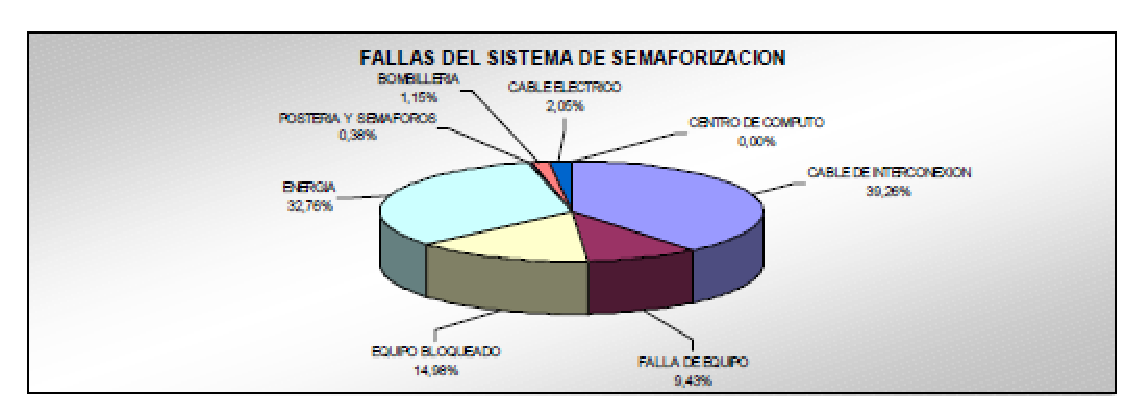
\includegraphics[width=1\textwidth]{ima/estadistica_php9hcqYv}
    \caption{Estadística promedio  de fallas del sistema de semaforización de Bogotá D.C. \cite{5}}
    \label{fig:mesh2}
\end{figure}

\section{Personal}
A nivel personal es un reto cumplir con las especificaciones solicitadas por la compañía, al igual cumplir con este 
proyecto significa mejorar la movilidad en los puntos en los cuales está enfocado el grupo JAMPIG.
  \chapter{Objetivos}

\section{Objetivo General}
Implementar uno de los protocolos de comunicación enfocados a las ITS (NTCIP, OCIT, SCATS) en uno de 
los módulos semafóricos tipo maestro del GRUPO JAMPIG, capaz de conectarse a través del espectro 
electromagnético para su monitorización y control a una central semafórica que posea el protocolo seleccionado.
\section{Objetivos Específicos}

\textbf{3.2.1} Analizar, estudiar y evaluar los protocolos de comunicación orientados a las ITS.
\\
\textbf{3.2.2} Seleccionar e implementar el estándar a utilizar.
\\
\textbf{3.2.3} Actualizar el firmware de la central de control para dar paso al protocolo seleccionado.
\\
\textbf{3.2.4} Verificar, ajustar e integrar los módulos existentes del dispositivo semafórico tipo maestro junto con el protocolo incorporado.
\\
\textbf{3.2.5} Validar la conexión del módulo semafórico tipo maestro del grupo JAMPIG a una central de control semafórica que trabaja bajo el protocolo utilizado.
  \chapter{Marco Teórico}
\section{Generalidades}
\subsection{ITS}
Los sistemas inteligentes de transporte pueden ser definidos como el matrimonio entre los avances 
en tecnologías de información y sistemas de comunicación con los vehículos y redes de caminos que 
forman parte del sistema de transporte. También pueden definirse como  la optimización de las 
funciones propias de los elementos básicos del Tránsito – Infraestructura Vial (calles y caminos) 
y Vehículos – mediante la aplicación de tecnologías avanzadas que interrelacionan tales elementos. \\

Existen dos elementos fundamentales en los Sistemas Inteligentes de Transporte  el primero es la 
capa lógica compuesta por las funciones y los procesos y el segundo es la capa física donde se 
encuentran los sistemas y las tecnologías. En ambos casos existe una coherencia con la definición 
de los servicios o aplicaciones ITS que se asocia a un marco normativo de referencia \cite{6}.
\begin{figure}[h]
    \centering
    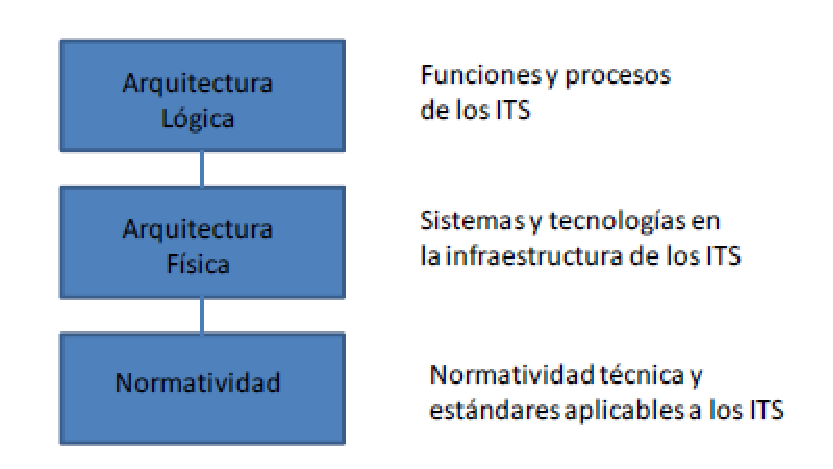
\includegraphics[width=1\textwidth]{ima/its_phpswxtBw}
    \caption{Estructura basica de los ITS. \cite{5}}
    \label{fig:mesh3}
\end{figure}
\subsection{Segmentos}
Caracterizados por su longitud, número de carriles, elemento de la red en el que comienza y elemento 
en el que finaliza. Sólo se considera un sentido de tráfico por segmento, por lo que una calle puede 
estar constituida por varios segmentos, tanto para expresar los dos sentidos de circulación (cuando 
ambos estén presentes) como las intersecciones que atraviesan \cite{7}.
\subsection{Intersecciones}
Son los elementos que principalmente definen los comienzos y finales de los segmentos, y está determinado 
por la unión de dos o más segmentos. Es aquí donde será necesario definir el derecho de paso de unos sentidos 
o direcciones respecto de otros, permitiendo realizar los cambios de dirección en el flujo de tráfico de una 
forma eficiente y segura\cite{7}.
\subsection{Flujo}
Es la cantidad de vehículos por unidad de tiempo en un determinado segmento[7].
\subsection{Velocidad}
Distancia recorrida por unidad de tiempo. La velocidad a la que circulan los vehículos es un dato importante 
para medir el nivel de congestión que existe\cite{7}.
\subsection{Tiempo}
Es el tiempo de viaje sobre un segmento del camino conocido. Esta medida es obtenida dividiendo el largo de 
la calle entre la velocidad media en recorrer la calle, en el caso de los vehículos, o en atravesarla, en el 
caso de los peatones\cite{7}.
\subsection{Ocupación}
Es el porcentaje de tiempo que en un segmento de una ruta es ocupado por vehículos\cite{7}.
\subsection{Densidad}
Es la cantidad de vehículos por unidad de distancia, en un periodo de tiempo\cite{7}.
\subsection{Funcionalidad de un semáforo}
\subsubsection{Operación constante}
Las indicaciones de rojo y verde son temporizadas a valores constantes calculados mediante el análisis del 
comportamiento histórico del tráfico en la intersección. Este tipo de operación asume que los patrones de 
tráfico pueden predecirse según sea la hora del día y, por lo tanto, no precisa de detectores de tráfico en 
la intersección que regulan. Este tipo de operación sólo suele ser utilizada cuando no se dispone de un presupuesto 
suficiente para implementar una operación flexible\cite{19}.
\subsubsection{Operación Flexible}
Las intersecciones que operan de esta manera consisten de controladores de tráfico y detectores de vehículos 
colocados en las vías próximas a la intersección. En una operación flexible se tiene que calcular la duración 
de los intervalos de verde. Los intervalos de verde pueden finalizar en una de las siguientes cuatro formas\cite{8}.
\paragraph{Alcance del tiempo máximo de tiempo verde (timing out)}
El intervalo se acaba cuando se alcanza un tiempo máximo de verde previamente establecido\cite{8}.
\paragraph{Disminución sensible del flujo de tráfico en las proximidades de la intersección (gapping out)}
Cuando se presenta un flujo ligero de tráfico que es menor que un cierto valor umbral previamente establecido\cite{8}.
\paragraph{Finalización por orden del sistema (force-off)}
Cuando un sistema de semáforos es parte de un sistema coordinado, el sistema mantiene la señal en espera con la 
operación indicada\cite{8}.
\paragraph{La señal es expulsada}
Cuando un vehículo prioritario, por ejemplo una ambulancia o un coche de bomberos, se aproxima a la intersección, 
los intervalos de verde asociados a movimientos no prioritarios deben de terminar en favor de los que están asociados 
a esos movimientos prioritarios\cite{8}.

\section{Software}
\subsection{Protocolos de comunicación enfocados al transporte}
\subsubsection{NTCIP (Estados Unidos)}
El NTCIP es un proyecto de estandarización conjunta de la AASHTO, ITE, y NEMA, Oficina del Secretario Adjunto de 
Investigación y Tecnología. NTCIP es una familia de estándares de comunicación para transmitir datos y mensajes 
entre el ordenador sistemas utilizados en los Sistemas de Transporte Inteligente (ITS). 
Un estándar de comunicaciones especifica un conjunto de reglas para los mensajes de cómo se codifican y se transmiten 
entre los dispositivos electrónicos. El equipo en cada final de una transmisión de datos utiliza la misma especificación 
para comunicarse con éxito. Es un poco como las lenguas del ser humano dado que tienen unas reglas para el alfabeto, 
vocabulario y gramática para un idioma especifico \cite{9}.
\subsubsection{SCATS (Australia)}
SCATS no requiere la intervención del operador para su funcionamiento del día a día. Sin embargo, los operadores tienen 
acceso instantáneo a la información de flujo de tráfico, estado del sistema y fallos hasta el nivel de una sola lámpara 
fundida. 
SCATS  se adapta a las exigencias de cambio de los flujos de tráfico. Por ejemplo, se puede adoptar una estrategia para 
eliminar las cargas de tráfico repentino e impredecible, tales como los cambios de clima, deportes y eventos públicos y 
conciertos.También supervisa las condiciones cambiantes de tráfico que se producen en el tráfico normal o especialmente 
cuando hay una avería, accidente u obras viales o condiciones meteorológicas adversas.Se ajusta continuamente a cambios 
de tiempo en la señal para optimizar el flujo por medición de la densidad de vehículos en cada carril \cite{10}.
\subsubsection{OCIT (Alemania)}
Significa interfaz abierta de sistemas de control de comunicación de tráfico, centro a centro. OCIT cubre las 
funciones para la comunicación entre los sistemas centrales de control de tráfico y el encaminamiento del tráfico, 
OCIT está orientado a las necesidades prácticas. Debido a los bajos costos de implementación, su uso también es adecuado 
para soluciones con presupuestos limitados \cite{11}.
\subsection{Protocolo ZIGBEE}
ZigBee es un estándar de comunicaciones inalámbricas diseñado por la ZigBee Alliance. Es un conjunto estandarizado de 
soluciones que pueden ser implementadas por cualquier fabricante. ZigBee está basado en el estándar IEEE 802.15.4 de redes 
inalámbricas de área personal (wireless  personal área Newark, WPAN) y tiene como objetivo las aplicaciones que requieren 
comunicaciones seguras con baja tasa de envío de datos y maximización de la vida útil de sus baterías\cite{12}.
\begin{figure}[h]
    \centering
    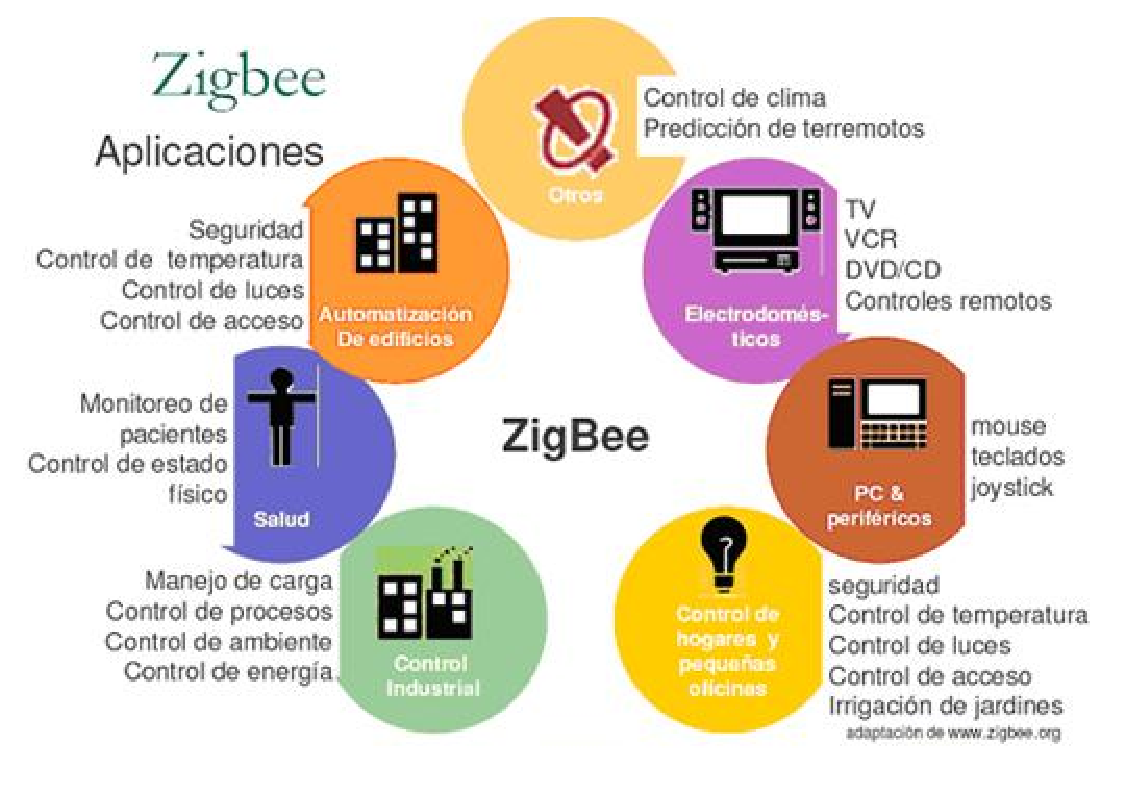
\includegraphics[width=1\textwidth]{ima/zb_phpI1D8AH}
    \caption{aplicaciones de la tecnologia ZIGBEE \cite{12}}
    \label{fig:mesh4}
\end{figure}
\section{Hardware}
\subsection{Antena GPRS}
Las siglas GPRS vienes de las palabras inglesas General Packet Radio Service( Servicio general de paquetes vía radio en 
castellano), la cual permite comunicarse vía satélite, sin necesidad de cables ni conexión física a dos terminales móviles. 
El GPRS permite pagar solo por la información enviada/recibida. Se basa en mandar la información en pequeños paquetes, es 
decir no enviar todo al mismo tiempo sino por tramas y únicamente cuando el canal estuviese libre, aprovechando así los 
huecos del mismo. Si la red está muy cargada, la trasmisión podría demorarse bastante\cite{13}.
\begin{figure}[h]
    \centering
    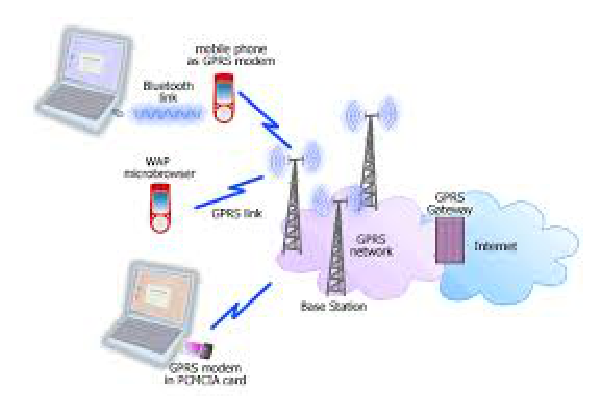
\includegraphics[width=1\textwidth]{ima/descarga_phpzcLdzH}
    \caption{Esquema de antena GPRS envío y recepción de información \cite{13}}
    \label{fig:mesh6}
\end{figure}
\subsection{Detectores de tráfico}
\subsubsection{Detectores de presión}
Consisten en una plancha de caucho en cuyo interior se sitúan dos láminas metálicas, muy cercanas entre sí, que establecen 
contacto cuando pasa un vehículo que supera un cierto peso umbral sobre la plancha. Todo este mecanismo está ubicado en la 
parte superior de una plataforma de hormigón o metálica que se empotra en el pavimento. Puede conseguirse una detección 
direccional si en vez de las dos láminas se ponen cuatro, enfrentadas dos a dos \cite{14}.
\subsubsection{Detectores magnéticos}
Detectan la distorsión del campo magnético producida por el paso sobre ellos de una masa metálica. Están formados por un 
tubo metálico en cuyo interior hay un núcleo de hierro con una bobina conectada a un amplificador. Los detectores más 
habituales que emplean esta tecnología no son capaces de detectar la dirección del movimiento, por lo que se fueron 
incorporando mejoras en su diseño dando lugar a los llamados detectores magnéticos compensados, formados por cuatro 
núcleos, que permiten distinguir el sentido de la marcha de la masa metálica que circula sobre ellos\cite{14}.
\subsubsection{Detectores de lazo}
Constituyen el tipo de detector más utilizado en las vías públicas actuales. Su principio de funcionamiento se basa en emplear 
las características de un lazo magnético situado sobre la superficie de la carretera y las fluctuaciones eléctricas producidas 
por la aproximación de un objeto metálico (que en este caso es un vehículo) para detectar su presencia y su paso. 

Efectivamente, mientras circula una corriente alterna por el lazo metálico situado sobre la carretera, se crea un campo magnético 
de la misma frecuencia cerca de la superficie de la carretera. Si un objeto metálico entra en este campo magnético, entonces la 
inducción magnética causa corrientes sobre el objeto metálico y como resultado se produce una variación en la impedancia a la 
salida del lazo magnético. Cuando se detecta un cambio de impedancia se detecta un vehículo. El cambio de inductancia provocado 
por el paso de vehículos varía según el tipo de vehículo. Este tipo de detectores son más sensitivos a vehículos pequeños que a 
vehículos de gran volumen. Entre las medidas que este tipo de detector de tráfico puede proporcionar destacan las siguientes:
\begin{itemize}
    \item Presencia de un vehículo.
    \item Tipo de vehículo (mediante el empleo de técnicas de reconocimiento de patrones es posible diferenciar entre seis o más tipos de vehículos).
    \item Velocidad del vehículo (mediante el uso de lazos dobles).
    \item Ocupación de los lazos.
    \item Intervalo de tiempo entre vehículos.
\end{itemize}

\subsubsection{Detectores de Radar.}
Constan de un aparato emisor y otro receptor de ondas electromagnéticas y generalmente se suspenden sobre la vía o se colocan 
lateralmente a ella. En la actualidad se emplean dos tipos de detectores de radar de microondas en las aplicaciones de 
gestión del tráfico. 
El primero transmite energía electromagnética a una frecuencia constante midiendo la velocidad de los vehículos dentro de su 
campo de visión usando el principio Dopler, en el que la diferencia de frecuencia entre las señales transmitidas y recibidas 
es proporcional a la velocidad del vehículo. Por lo tanto, la detección de una variación en la frecuencia denota el paso de un vehículo. 
Este tipo de sensor no puede detectar vehículos parados y, por lo tanto, no es adecuado para aplicaciones que precisan detectar 
la presencia de vehículos tales como regulación de semáforos o líneas de parada obligatoria. 
El segundo tipo de detector de radar de microondas transmite una onda en forma de diente de sierra, también denominada onda continua 
modulada en frecuencia, que varía la frecuencia transmitida de forma continua en el tiempo. Los vehículos parados se detectan midiendo 
el rango desde el detector hasta el vehículo y también calculando la velocidad del vehículo midiendo el tiempo que le lleva al vehículo 
viajar entre dos marcas internas que representan distancias conocidas para el radar. Al disponer de la característica de detección de 
vehículos parados, este detector suele denomina se radar de microondas de presencia real\cite{14}.
\subsubsection{Detector pasivo de infrarrojo}
Este tipo de dispositivo es capaz de detectar el paso y la presencia de vehículos, pero no su velocidad. 
Su método de funcionamiento se basa en un detector sensitivo a la energía de fotones colocado en un plano focal para medir la energía 
infrarroja emitida por los objetos en el campo de visión del detector. Los detectores pasivos no transmiten energía por si mismos. 
Cuando un vehículo entra en la zona de detección produce un cambio en la energía medida normalmente desde la superficie de la vía en 
la ausencia de vehículos. El cambio en la energía es proporcional a la temperatura absoluta del vehículo y la emisividad de la 
superficie metálica del vehículo (la emisividad es el cociente de la energía emitida respecto al radiante perfecto de energía a la misma 
temperatura). 
La diferencia de energía que es capaz de detectar este detector se reduce ante condiciones meteorológicas adversas 
(lluvia, nieve, niebla,...)\cite{14}.
\subsubsection{ Detector activo de infrarrojo}
Su funcionamiento es similar al de los detectores de radar por microondas. Los más comunes utilizan un diodo láser para emitir energía 
en el espectro cercano al infrarrojo, una porción del cual vuelve al receptor del detector desde el vehículo de su campo de visión. 
Los detectores basados en el radar láser pueden suministrar la presencia, el paso y la velocidad de vehículos. 
La medición de la velocidad se realiza anotando el tiempo que le lleva a un vehículo cruzar dos haces de infrarrojos que están ubicados 
a una distancia conocida. Algunos de estos detectores son capaces de clasificar los vehículos contrastando las mediciones con unos 
ficheros modelos \cite{14}.
\subsubsection{Detectores de ultrasonido}
Los detectores ultrasónicos emiten sonidos a una frecuencia entre los 25 kHz a los 50 kHz (según sea el fabricante). 
Estas frecuencias no están en la franja audible. Una porción de la energía transmitida se refleja desde la carretera o la superficie 
del vehículo de nuevo al detector y se procesa para dar el paso y presencia de vehículos. Un detector típico de presencia ultrasónico 
emite energía ultrasónica en forma de pulsos. El tiempo que le lleva al pulso dejar el detector, chocar contra la superficie y regresar 
al detector es proporcional al rango del detector a la superficie. Cuando un vehículo se introduce en su campo de visión se mide el rango 
desde el detector hasta el vehículo, obteniéndose un rango menor que el producido sobre la vía lo que produce en el detector una señal 
de detección de vehículo \cite{14}.
\subsubsection{ Detectores acústicos pasivos}
El tráfico de vehículos produce una energía acústica o sonido audible desde una variedad de fuentes dentro del vehículo y desde la 
interacción de los neumáticos del vehículo con la superficie de la vía. Cuando un vehículo pasa por la zona de detección, el algoritmo 
de procesado de señales detecta un incremento respecto a la energía del sonido y se genera una señal de presencia de vehículo. 
Cuando el vehículo abandona la zona de detección, la energía del sonido decrece hasta por debajo de un nivel de detección umbral 
terminando la señal de presencia de vehículo\cite{14}.
\subsubsection{Procesadores de imágenes de video}
Estos detectores identifican los vehículos y sus parámetros de flujo de tráfico asociados mediante el análisis de las imágenes 
suministradas por cámaras de vídeo. Estas imágenes se digitalizan y se analizan para identificar los cambios observables entre 
imágenes sucesivas, es decir, los cambios de los niveles de contraste entre píxeles adyacentes. Por lo tanto estos detectores 
pueden suministrar información sobre el paso, presencia, velocidad, longitud y cambios de carriles de vehículos según sea el 
tipo de técnica de procesado de imágenes utilizada\cite{14}.
\begin{figure}[h]
    \centering
    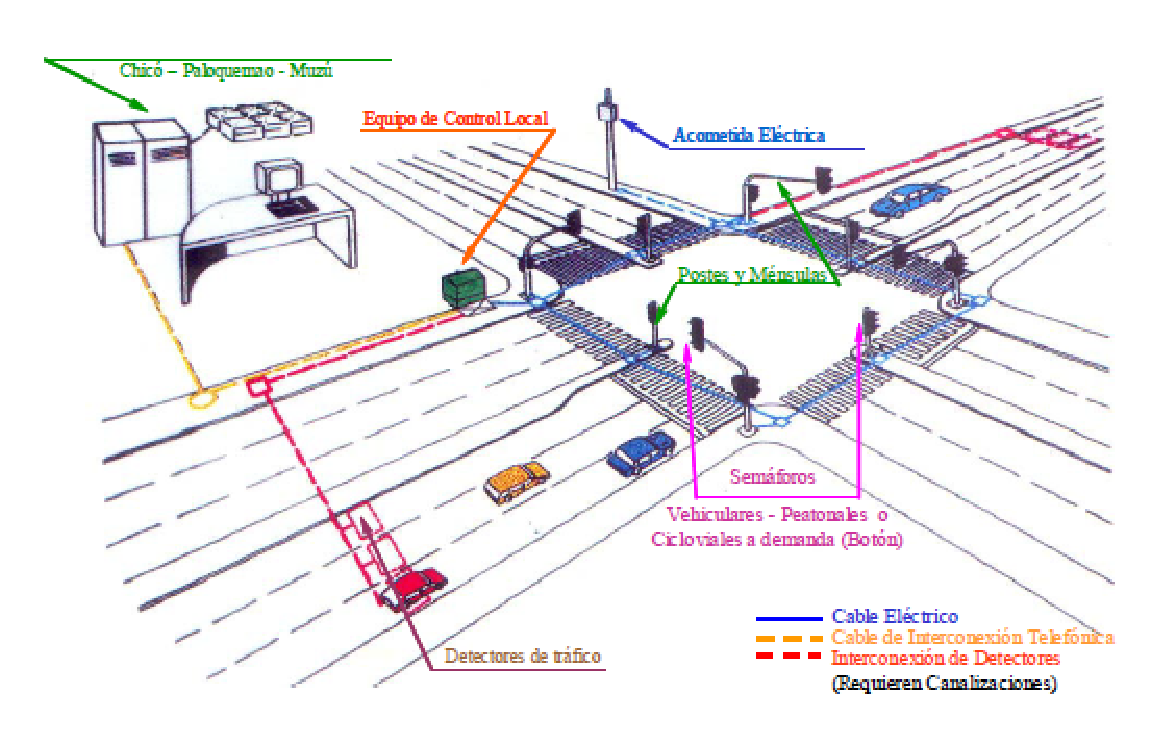
\includegraphics[width=1\textwidth]{ima/ca_phpB1BaNG}
    \caption{Configuración  típica de gestión de tráfico. Conexión del centro de control con una inetrsección semaforizada para Bogotá D.C. \cite{5}}
    \label{fig:mesh5}
\end{figure}
  \chapter{Estado del Arte}
La evolución de los sistemas de semaforización inteligente en los últimos años ha sido de forma exponencial, lo que trae nuevas tecnologías, nuevos paradigmas, nuevos prototipos y nuevos esquemas, en este documento se analizará los protocolos de comunicación enfocados a la movilidad vehicular, para luego centrarce en solo los protocolos NTCIP, SCATS, y OCIT; al igual se enfoca a tecnologías de energías renovables, puesto que el modulo planteado trabaja bajo esquemas de energía solar, otra de las tecnologías trabajadas es la tecnología ZIGBEE.

\section{El sistema SCOOT}
(Técnica de Optimización de los valores de Desplazamiento, Ciclo y Giro) se fundamenta en la experiencia aportada por la Red de Tráfico TRANSYT. Lo positivo de este sistema es que realiza una optimización a tres niveles: giro, ciclo y desplazamiento. Utiliza los datos de los detectores de desplazamiento, normalmente detectores de lazo enterrados en el pavimento. Mide el tráfico en tiempo real y desarrolla un modelo de flujo de demanda a cada intersección. Esta secuencia se contrasta con el flujo de salida y de vehículos encolados. Los ajustes temporales son pequeños y no se adaptan a los picos de tráfico, salvo que sea un aumento continuo. Este modelo es utilizado en grandes urbes como Toronto, Madrid, Reino Unido, y para el caso colombiano en Cartagena\cite{15}.

\section{El sistema SCATS}
Se compone de tres niveles, un computador central para realizar la monitorización del sistema global, computadores regionales remotos o locales y controladores locales de señales de tráfico. Su objetivo es la reducción de paradas y retraso, mejorando los tiempos de las rutas. 
El computador central permite el acceso a los computadores regionales para la  recogida de datos de tráfico, datos de entrada y acciones de monitorización.\cite{15}.
\begin{figure}[h]
    \centering
    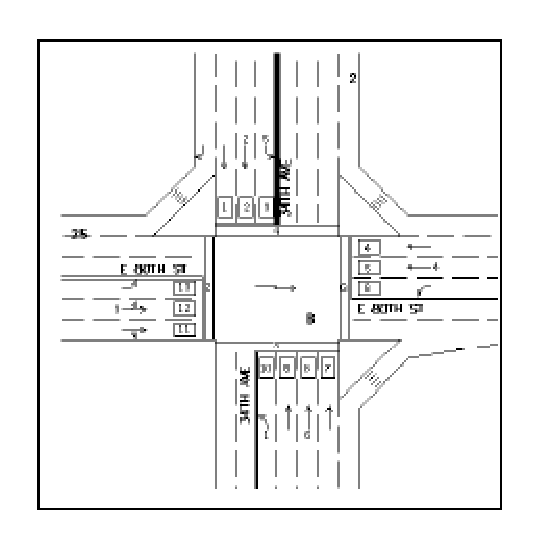
\includegraphics[width=0.4\textwidth]{ima/cruce_phpcUjY57}
    \caption{Sensores para sistema SCATS \cite{18}}
    \label{fig:mesh7}
\end{figure}

\begin{figure}[h]
    \centering
    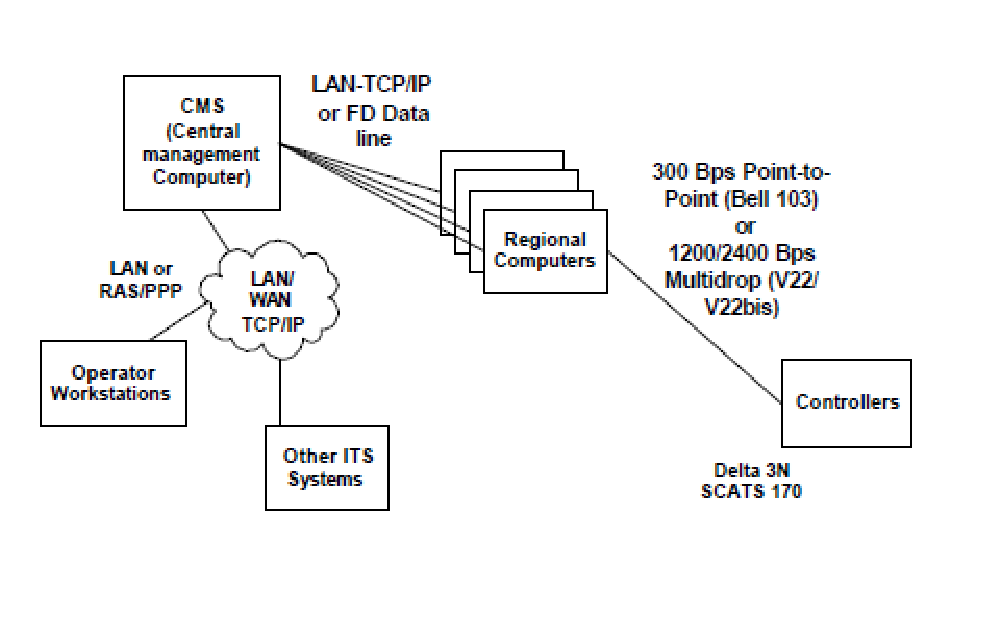
\includegraphics[width=0.8\textwidth]{ima/scat_php1eUteh}
    \caption{Esquema Básico del protocolo SCATS \cite{18}}
    \label{fig:mesh8}
\end{figure}
\section{Sistema NTCIP} 
Dicho sistema cuenta con varias versiones sobre el mismo desarrollo, fue implementado por compañías estadounidenses, dentro del mismo país, este sistema cuenta con varias características:
\subsection{Interoperabilidad}
La interoperatividad refleja la capacidad de múltiples sistemas y dispositivos de diferentes tipos de centros de intercambio información para un propósito común. La interoperabilidad permite que los componentes del sistema de diferentes  proveedores para comunicarse entre sí para proporcionar las funciones del sistema y para trabajar juntos como un sistema completo. Por ejemplo, utilizando la infraestructura mismas comunicaciones para interconectar un sistema de gestión con el tráfico controladores de señal, señales de mensajes dinámicos, controles de vigilancia de vídeo y otros dispositivos para gestionar el tráfico refleja un ejemplo real mundo de interoperabilidad.
\subsection{Intercambiabilidad}
La intercambiabilidad refleja la capacidad de intercambiar dispositivos del mismo tipo en la misma canal de comunicaciones y que dichos dispositivos interactuar con otros dispositivos del mismo tipo que utiliza funciones basadas en estándares. Con capacidad de intercambio, los componentes del sistema pueden modificarse a cabo (conmutada) con componentes similares de diferentes fabricantes, ya que poseen común funcional y física características. Un ejemplo de intercambiabilidad es un controlador de señales de diferentes fabricantes que interactúan entre sí para  proporcionar la coordinación de señales de tráfico a lo largo de un camino pasante arterial[16]. 
\subsection{Centro de Campo (C2F) Comunicaciones}
NTCIP proporciona estándares de comunicaciones de dos tipos diferentes para sus comunicaciones. El primer tipo es entre un sistema central y  múltiples dispositivos de control o de vigilancia gestionado por la central. Un ejemplo de un sistema central es un ordenador en el seguimiento  y el control de la operación de controladores basados en microprocesadores de carretera para las señales de tráfico dentro de una ciudad. El sistema central puede enviar instrucciones a los controladores de semáforos para cambiar configuraciones de cronometraje, las condiciones de circulación y el envio de información de  los estados del tráfico a la computadora. Otros ejemplos de este tipo de comunicaciones incluyen.
\begin{itemize}
    \item Un sistema de transporte a bordo del vehículo se comunica con un dispositivo de señales de tráfico para facilitar la prioridad de tránsito.
    \item  Un sistema de gestión de la autopista que comunica con los detectores y medidores de rampa en las autopistas.
    \item El control de sistema de gestión de tráfico de un camino de iluminación, circuito cerrado de televisión (CCTV), las señales de mensajes dinámicos, transmisores de radio de asesoramiento, sensores ambientales y estaciones de volumen de tráfico en las carreteras. 
\end{itemize}
Como la mayoría de aplicaciones de este tipo implican un sistema de centro de la comunicación con varios dispositivos en la carretera o en los  vehículos de la agencia, este tipo de comunicación se denomina "centro de campo" (C2F). Los protocolos NTCIP destinados a esta aplicación se utiliza a menudo en un entorno donde un sistema de centro, rutinariamente encuesta cada dispositivo de campo, como en el caso más común de múltiples dispositivos de campo, se suele compartir un canal de comunicaciones.
\subsection{Centro de Centro de Comunicaciones (C2C)}
El segundo tipo de comunicación implica los mensajes enviados entre dos o más sistemas de centro. Este tipo de comunicación se denomina centro a centro de comunicaciones (C2C), aunque dos o más de los diversos sistemas pueden de hecho, estar situados dentro de la misma "central" o edificio, son lógicamente separados. C2C implica comunicaciones de igual a igual entre cualquier número de sistemas de centros en un muchos a muchos de una red. Este tipo de comunicación es similar a la Internet, en que cualquier centro puede solicitar información de, o proporcionar información a, cualquier número de otros centros. Un ejemplo de las comunicaciones C2C es de dos centros de gestión de tráfico que intercambian en tiempo real información sobre el inventario y el estado de los dispositivos de control de tráfico. Esto permite que cada sistema de centro sabe qué plan de tiempo, por ejemplo, el otro sistema central está en marcha para permitir la coordinación de señales de tráfico allá de las fronteras geográficas del centro \cite{16}.

\begin{figure}[H]
    \centering
    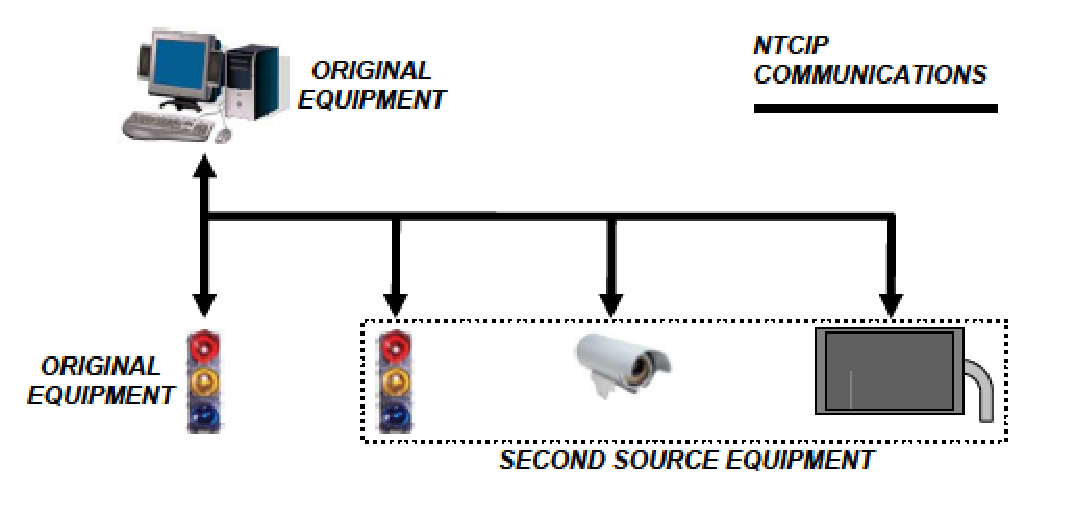
\includegraphics[width=1\textwidth]{ima/ntc_php4gbMlF}
    \caption{Propiedades e imteroperatividad e intercambiabilidad de NTCIP\cite{9}}
    \label{fig:mesh9}
\end{figure}
\begin{figure}[H]
    \centering
    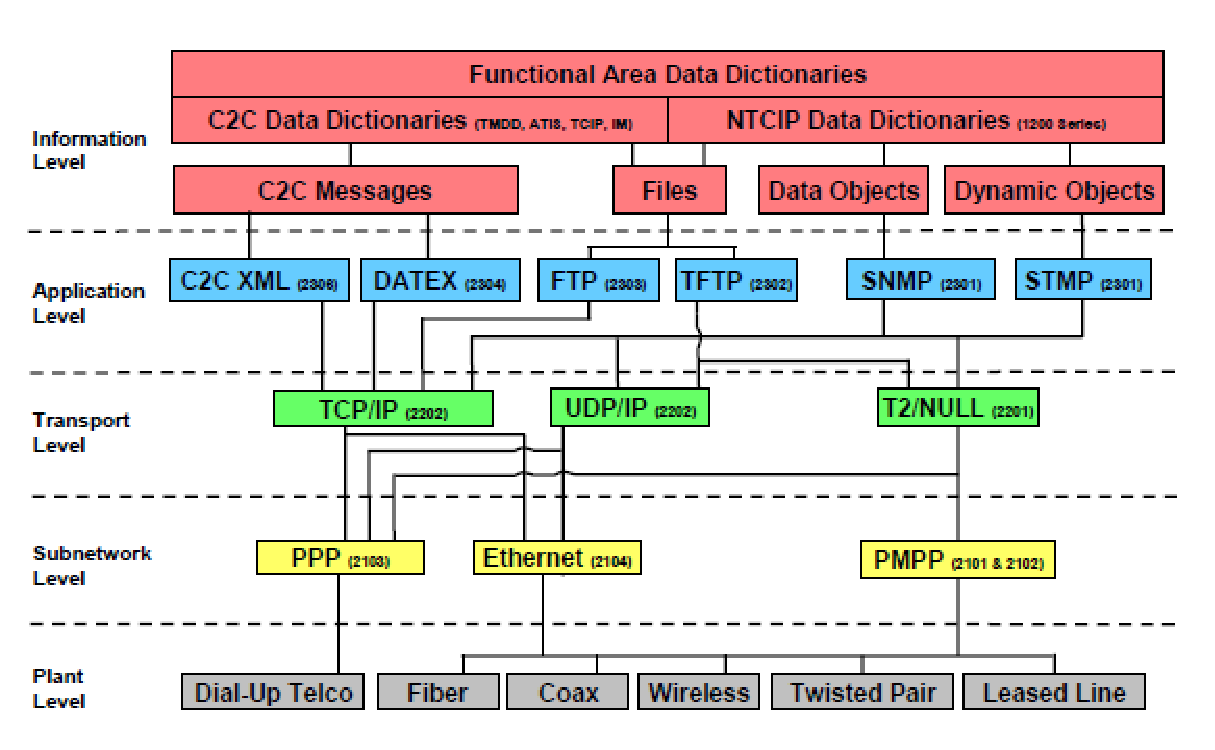
\includegraphics[width=0.8\textwidth]{ima/ntc1_phpfqEM84}
    \caption{NTCIP Framework \cite{9}}
    \label{fig:mesh10}
\end{figure}
\begin{figure}[H]
    \centering
    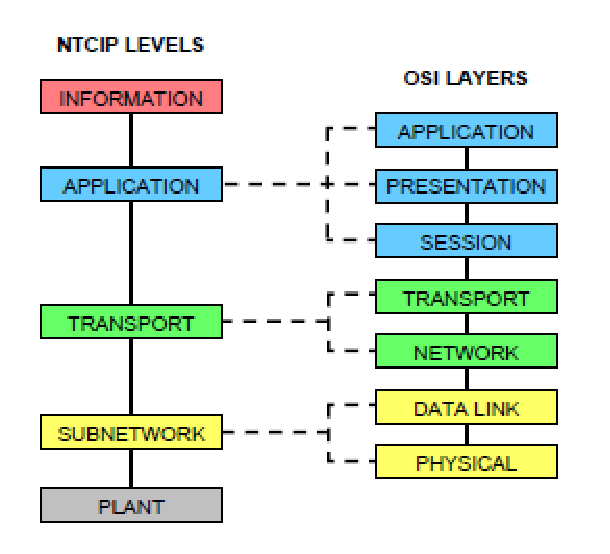
\includegraphics[width=0.6\textwidth]{ima/ntc2_phpj0fRQP}
    \caption{Mapa capas OSI a capas NTCIP \cite{9}}
    \label{fig:mesh11}
\end{figure}
\newpage
\newpage


\section{Sistema OCIT}
Para el sistema OCIT el cual fue incorporado en algunas ciudades de Alemania, se tienen las siguientes características:
\begin{itemize}
    \item Protocolo de conversión basado en el estándar SOAP con un simple patrón de petición-respuesta en la comunicación (recuperación directa de los datos).
    \item Definición de un modelo de datos global en la región de datos de proceso que abarca todas las ramas del sistema de enrutamiento de control de tráfico y el tráfico, el uso de la OCIT-I modelo de datos para los SAT. La funcionalidad del modelo de datos de la OCIT-I es retratado en su totalidad.
    \item Integración de sistemas y los ajustes deseados se regulan previamente como parte de la planificación del proyecto.
    \item Pruebas de conformidad del protocolo se llevan a cabo en un entorno de prueba que se proporciona el uso de OCIT. Las pruebas de todas las implementaciones de protocolo (contenido y datos) se llevan a cabo sobre una base de proyecto por proyecto.
    \item Las actualizaciones incluyen componentes de DATEX II pueden ser posibles dependiendo de retomar proyecto de requisitos.
    \item Las actualizaciones incluyen componentes de DATEX II pueden ser posibles dependiendo de retomar proyecto de requisitos.
    
\end{itemize}

 La interfaz de comunicación debe aplicarse de la misma manera en todas las unidades centrales. Para ello, el protocolo SOAP se utiliza como una interfaz de comunicación de nivel superior, a través de la cual toda la comunicación se lleva a cabo. La forma descrita aquí se designa como un protocolo OCIT-C.
 Esta interfaz OCIT-C está abierta y se puede utilizar en diversos sistemas, en su mayor parte en el área de los sistemas de control de tráfico. Es el propósito de este documento para describir el protocolo OCIT-C y su uso. No se va a describir los datos estructurales de los datos a transmitir. Esto se describe en el documento "OCIT-C de datos".
 Este sistema se incorpora bajo el siguiente esquema de conexión y de interactividad \cite{17}.
 \begin{figure}[h]
    \centering
    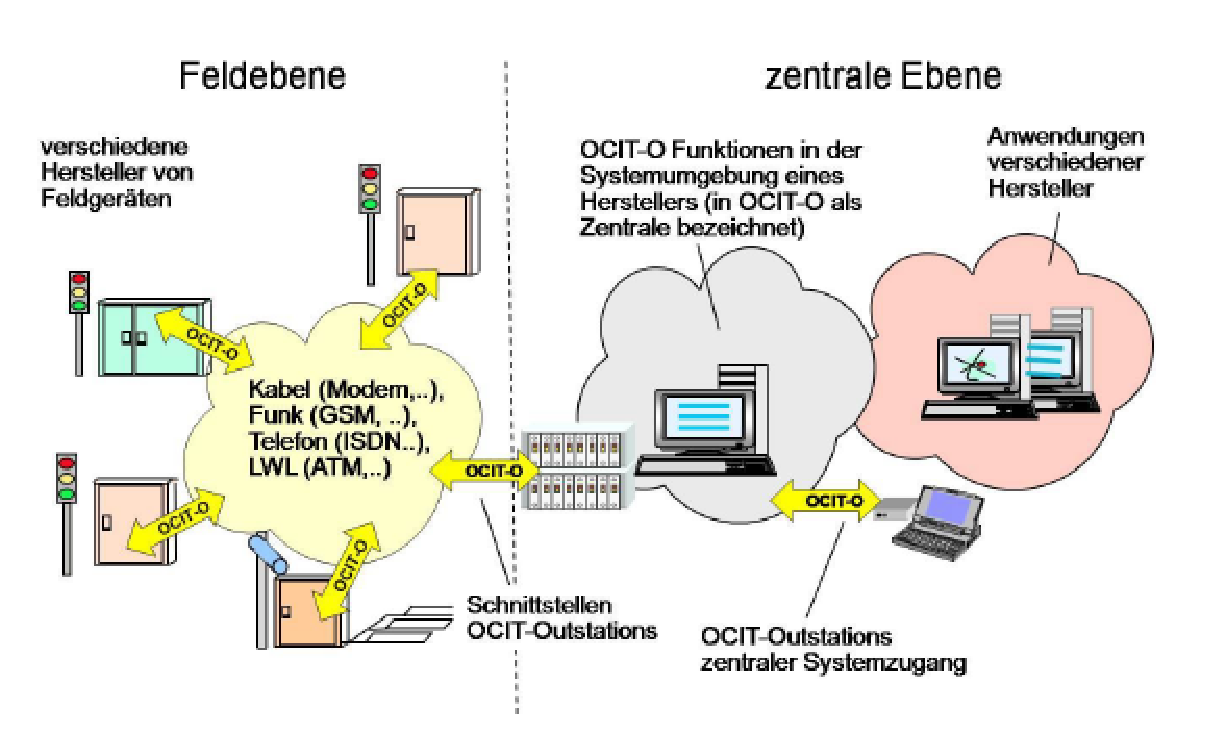
\includegraphics[width=1\textwidth]{ima/ocit_php7K8DbI}
    \caption{Esquema general de OCIT-C \cite{11}}
    \label{fig:mesh12}
\end{figure}
 El siguiente gráfico muestra como se comunica los servidores con los clientes, siendo una interactividad de tipo bidireccional.
 \begin{figure}[h]
    \centering
    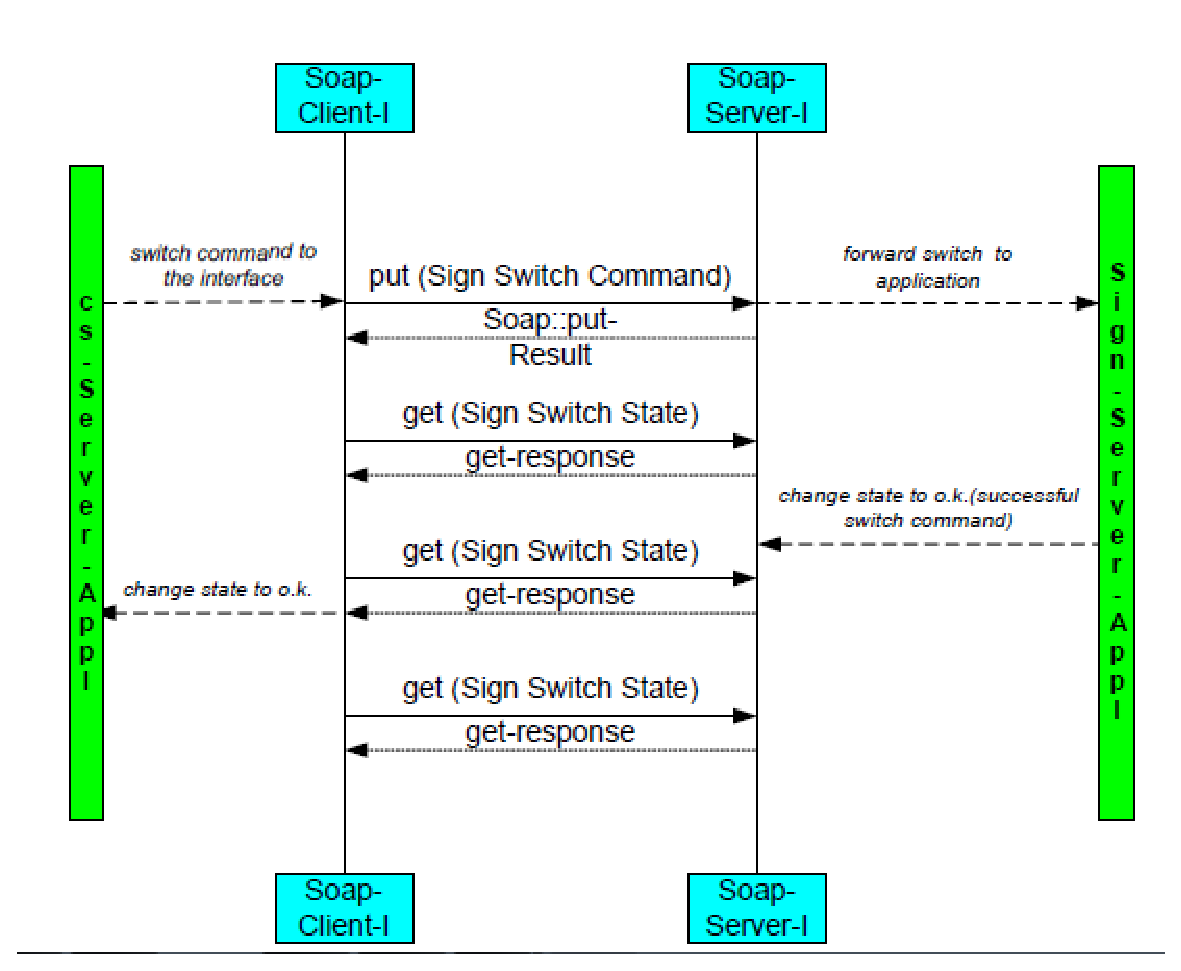
\includegraphics[width=0.8\textwidth]{ima/ocit1_phpVmReMk}
    \caption{Estado regular de la comunicación \cite{17}}
    \label{fig:mesh13}
\end{figure}
 En resumidas cuentas y palabras el protocolo se describe como 4 capas, al estilo del protocolo OSI\cite{17}.

\begin{figure}[h]
    \centering
    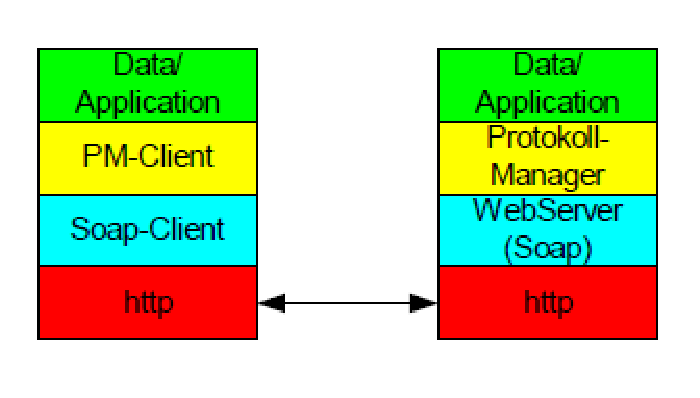
\includegraphics[width=0.6\textwidth]{ima/ocit2_phplDTo60}
    \caption{Capas cliente- servidor OCIT-C \cite{17}}
    \label{fig:mesh14}
\end{figure}
\newpage
\section{Tecnología ZBEE}
ZigBee, también conocido como "HomeRF Lite", es una tecnología inalámbrica con velocidades comprendidas entre 20 kB/s y 250 kB/s.· Los rangos de alcance son de 10 m a 75 m\cite{12}.
\begin{itemize}
    \item Puede usar las bandas libres ISM (6) de 2,4 GHz (Mundial), 868 MHz (Europa) y 915 MHz (EEUU).
    \item  Una red ZigBee puede estar formada por 255 nodos los cuales tienen la mayor parte del tiempo el transceiver ZigBee dormido con objeto de consumir menos energía que otras tecnologías inalámbricas.
    \item Un sensor equipado con un transceiver ZigBee pueda ser alimentado con dos pilas AA durante al menos 6 meses y hasta 2 años.
    \item La fabricación de un transmisor ZigBee consta de menos circuitos analógicos de los que se necesitan habitualmente.
    \item  Diferentes tipos de topologías como estrella, punto a punto, malla, árbol.
    \item Acceso de canal mediante CSMA/CA(7) (acceso múltiple por detección de portadora con evasión de colisiones).
    \item Escalabilidad de red -- Un mejor soporte para las redes más grandes, ofreciendo más opciones de gestión, flexibilidad y desempeño.
    \item  Fragmentación -- Nueva capacidad para dividir mensajes más largos y permitir la interacción con otros protocolos y sistemas.
    \item  Agilidad de frecuencia -- Redes cambian los canales en forma dinámica en caso que ocurran interferencias.
    \item Gestión automatizada de direcciones de dispositivos.
    \item  El conjunto fue optimizado para grandes redes con gestión de red agregada y herramientas de configuración.
    \item Localización grupal -- Ofrece una optimización adicional de tráfico necesaria para las grandes redes.
    \item  Instalación de servicio inalámbrico -- El modulo fue mejorado con capacidades para poner en marcha el servicio inalámbrico.
    \item Recolección centralizada de datos -- El modulo fue sintonizado específicamente para optimizar el flujo de información en las grandes redes.    
\end{itemize}
    
\subsubsection{Ventajas}
\begin{itemize}
\item Ideal para conexiones punto a punto y punto a multipunto.
\item Diseñado para el direccionamiento de información y la actualización de la red.
\item  Opera en la banda libre de ISM 2.4 Ghz para conexiones inalámbricas.
\item  Óptimo para redes de baja tasa de transferencia de datos.
\item  Alojamiento de 16 bits a 64 bits de dirección extendida.
\item  Reduce tiempos de espera en el envío y recepción de paquetes.
\item  Detección de Energía (ED).
\item  Ciclo de trabajo mínimo - Proporciona larga duración de la batería.
\item  Soporte para múltiples topologías de red: Estática, dinámica, estrella y malla.
\item Hasta 65.000 nodos en una red.
\item  Cifrado AES de 128-bit - Provee conexiones seguras entre dispositivos.
\item Son más baratos y de construcción más sencilla.
\end{itemize}
\subsubsection{Desventajas}
\begin{itemize}
\item La tasa de transferencia es muy baja.
\item Solo manipula textos pequeños comparados con otras tecnologías.
\item Zigbee trabaja de manera que no puede ser compatible con bluetooth en todos sus aspectos porque no llegan a tener las mismas tasas de transferencia, ni la misma capacidad de soporte para nodos.
\item  Tiene menor cobertura porque pertenece a redes inalámbricas de tipo WPAN\cite{12}.
\end{itemize}
\begin{figure}[h]
    \centering
    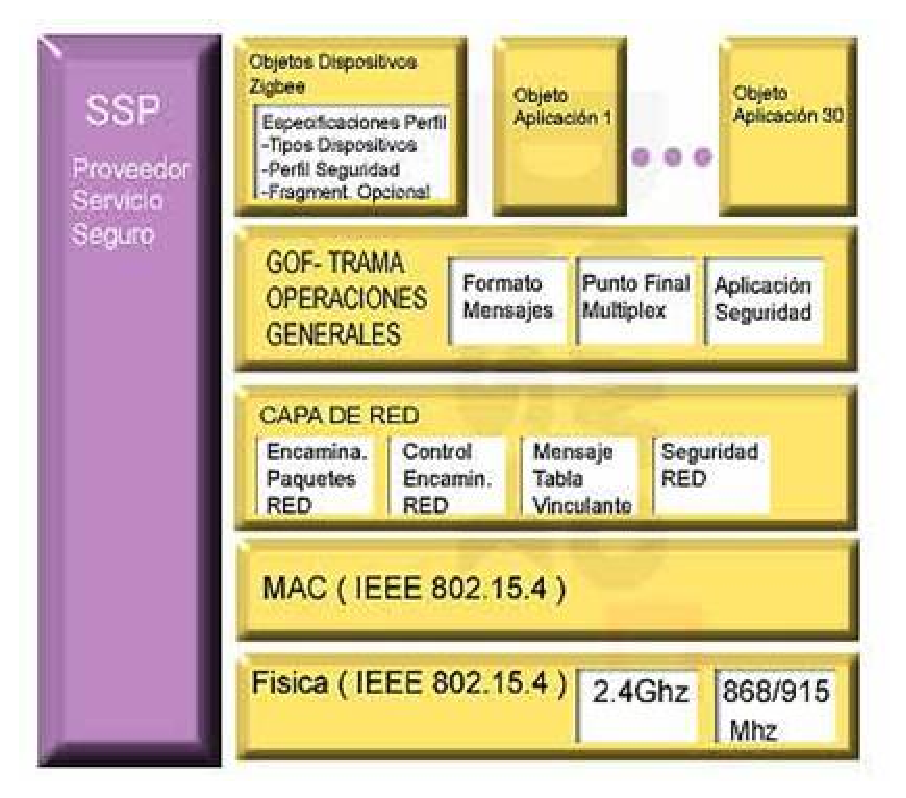
\includegraphics[width=1\textwidth]{ima/z1_phpBkhYj6}
    \caption{Estructura ZIGBEE \cite{12}}
    \label{fig:mesh15}
\end{figure}
  \chapter{Metodología}

Para el desarrollo del presente proyecto se trabajarán diferentes fases basadas en cada uno de los objetivos a ejecutar.

\section {Fase I}

Para mejorar un proceso ya implementado, lo primero que se debe plantear es una investigación rigurosa con respecto a todas las variables tenidas en cuenta en dicho proceso, de manera que quede cubierta cada una de las posibilidades de aquello que se debe y puede mejorar; por este motivo, lo primero que se efectuará será el estudio y evaluación de cada uno de los procesos a optimizar, para ello se estudiarán las encuestas realizadas por los organismos de tránsito existentes, si la información aportada no es suficiente para el proyecto,se realizarán encuestas para cumplir con el objetivo, así mismo se evaluarán todos los índices posibles y apropiados con respecto a la movilidad evaluada, métodos de desarrollo y las tecnologías que se pueden implementar.
\subsection{Investigación exhaustiva sobre las ITS' }

Para reconocer la forma en que operan los semáforos en la actualidad se hace necesario, estudiar su evolución y en este concepto entra todo aquello relacionado a las TIC's.
Para esta actividad se estudiará acerca de lo relacionado a tecnologías inteligentes enfocadas al transporte; indagando en los lugares donde se han puesto en marcha estos sistemas y realizando análisis de esta información.  

%Lo primero que se hará sera analizar todas las variables que se pueden generar con respecto a los sistemas de transito, se evaluaran las apropiadas y posibles encuestas, índices, estadísticas y opiniones respecto a este ámbito, con la finalidad de obtener la mayor cantidad de información posible referente al funcionamiento de dichos sistemas.
\subsection{Determinación del modo de encriptación de la información}
Puesto que se esta manejando información a la que no cualquiera debe tener acceso se hace necesario encriptar los datos a enviar; para esto se realizará un estudio de las formas de proteger información que existen en la actualidad para seleccionar el más apropiado.

\subsection{Preparación y análisis teórico}

Para desarrollar una idea, es necesario conocer a fondo todas las maneras en que se puede abordar dicha idea, por lo tanto, esta fase del proyecto sera muy importante, puesto que se llevará a cabo una profunda documentación con respecto a todos los métodos que pueden ser implementados.

Se evaluará cada unos de los protocolos que pueden ser implementados en los procesos de las ITS'; centrándose en los estándares NTCIP, SCATS y OCIT, dado que estos han sido utilizados en el país; en esta etapa se realizarán análisis de factores como información al respecto, tendencia de implementación y la justificación del uso de los ya mencionados estándares, en pocas palabras realizar un cuadro comparativo entre pros y con-tras de cada estándar para así avanzar descartar ó establecer el indicado.
    
\section {Fase II}

Con respecto a la movilidad del medio a mejorar; teniendo en cuenta los estudios realizados anteriormente, se escogerán los métodos apropiados de monitoreo a implementar para que el sistema tome las decisiones apropiadas en tiempo real, con respecto a las finalidades deseadas.

\subsection{Elección de métodos}

Elegir uno de los protocolos anteriormente enunciados, con respecto a las necesidades planteadas y los alcances de los empleadores, de manera apropiada, es una de las decisiones mas importantes a tomar, puesto que esta es la finalidad del objetivo general del proyecto, de manera que no se escatimara en recursos al momento de efectuar esta fase. Se estudiarán dichos protocolos los mas profundamente posible para definir cual sera implementado, realizando las respectivas pruebas.


\subsection{Implementación del protocolo}

Ya escogido y probado el protocolo a ejecutar, sera implementado y asi, se adaptara este a la antena GPRS que se utilizará, actualizando el controlador que actualmente maneja la compañía .

\section {Fase III}

\subsection{Modificación software }

Puesto que solo se trabajará sobre la comunicación entre el módulo y la central de operación es necesario modificar el software de la central para que tome la información procedente de la antena GPRS y le desarrolle un tratamiento tal que muestre en pantalla justo lo que se envió desde el módulo. 

%Con el fin de mejorar los procesos ya planteados, se procederá a implementar una plataforma web para el monitoreo de los controladores enunciados anteriormente, mediante protocolos y tecnologías  óptimas.


%Se elegirá de manera correcta los sistemas apropiados, para disminuir los tiempos de espera. Se desarrollaran herramientas mas amigables que faciliten el control y la supervisión de los sistemas de transito. 

\section {Fase IV}

Ya habiendo sido implementados todos los conceptos de desarrollo general del proyecto, se procederá a incorporar todos los módulos en uno solo.

\subsection{Verificación y ajuste del modulo RF}
Dado que este módulo ya existe, solo se plantea esta actividad para corroborar su funcionalidad, en caso de algún error o falla se ajustará a las necesidades del proyecto.

\subsection{Verificación y ajuste de sistema de potencia}

Uno de los aspectos fuertes del sistema radica en que la fuente de alimentación(voltaje) se realiza de forma autónoma, es decir se  utiliza paneles fotovoltaicos y se realiza toda una etapa de potencia para suministrar la energía eléctrica necesaria para el funcionamiento de los demás módulos; en este proceso solo se verificara que su funcionamiento sea el adecuado y en caso de algún error o falla se ajustará a las necesidades de este proyecto.


\subsection{Verificación y ajuste del modulo LAN}

En esta etapa se corroborará que la comunicación entre los dispositivos XBEE funcione como han venido trabajando y al igual que en las fases anteriores en caso tal de encontrar un error se procede a repararlo.

\section {Fase V}

Como todo proyecto lo demanda, la fase siguiente corresponde a la materialización de todo diseño efectuado anteriormente. 

\subsection{Programación inicial}

En esta etapa se configurará el primer plan de trabajo del semáforo, a través de la comunicación preparada entre el modulo y la central de control de la compañía.
\subsection{Verificación conexión con central existente }

Dado que uno de los objetivos es comprobar el funcionamiento del protocolo, se realizarán pruebas de conexión, es decir lograr enviar y recibir información desde el módulo hasta una central que ya posee el protocolo seleccionado en etapas anteriores.
Por lo dicho anteriormente la cuestión radica en realizar el mismo tipo de funcionamiento que se opera entre el módulo y la central de la compañía sino ahora entre el modulo y una central mucho más grande.

\subsection{Pruebas de calidad del sistema}


Ya instalado el sistema ITS, se harán las respectivas pruebas de calidad. Esperando que del sistema responda de manera óptima para concluir con el trabajo de manera exitosa y satisfactoria para todas las partes involucradas.
  \chapter{Cronograma}
\section{Fase I}
\begin{table}[h]
  \centering
  \label{my-label}
  \begin{tabular}{|l|l|l|l|l|l|l|l|l|}
    \hline
    \multicolumn{9}{|c|}{\cellcolor[HTML]{F8FF00}{\color[HTML]{000000} Fase I}}                                                                                                                                                                                                                          \\ \hline
    \multicolumn{1}{|c|}{}                                                                                                 & \multicolumn{4}{l|}{Mes 1} & \multicolumn{4}{l|}{Mes 2}                                                                                                                     \\ \cline{2-9}
    \multicolumn{1}{|c|}{\multirow{-2}{*}{Actividad}}                                                                      & 1                          & 2                          & 3                        & 4                        & 1                        & 2                        & 3 & 4 \\ \hline
    \begin{tabular}[c]{@{}l@{}}Investigación exhaustiva ITS'\end{tabular}                                                  & \cellcolor[HTML]{3166FF}   &                            &                          &                          &                          &                          &   &   \\ \hline
    \begin{tabular}[c]{@{}l@{}}Determinación de factores para la\\  toma de decisiones por parte\\ del modulo\end{tabular} &                            & \cellcolor[HTML]{3166FF}   & \cellcolor[HTML]{3166FF} &                          &                          &                          &   &   \\ \hline
    Análisis de protocolo NTCIP                                                                                            & \cellcolor[HTML]{3166FF}   & \cellcolor[HTML]{3166FF}   & \cellcolor[HTML]{3166FF} & \cellcolor[HTML]{3166FF} & \cellcolor[HTML]{3166FF} & \cellcolor[HTML]{3166FF} &   &   \\ \hline
    Análisis de protocolo OCIT                                                                                             & \cellcolor[HTML]{3166FF}   & \cellcolor[HTML]{3166FF}   & \cellcolor[HTML]{3166FF} & \cellcolor[HTML]{3166FF} & \cellcolor[HTML]{FFFFFF} & \cellcolor[HTML]{FFFFFF} &   &   \\ \hline
    Análisis de protocolo SCATS                                                                                            & \cellcolor[HTML]{FFFFFF}   & \cellcolor[HTML]{FFFFFF}   & \cellcolor[HTML]{FFFFFF} & \cellcolor[HTML]{FFFFFF} & \cellcolor[HTML]{3166FF} & \cellcolor[HTML]{3166FF} &   &   \\ \hline
    Documentación                                                                                                          & \cellcolor[HTML]{34FF34}   & \cellcolor[HTML]{34FF34}   & \cellcolor[HTML]{34FF34} & \cellcolor[HTML]{34FF34} & \cellcolor[HTML]{34FF34} & \cellcolor[HTML]{34FF34} &   &   \\ \hline
  \end{tabular}
  \caption{Fase I}
\end{table}



\section{Fase II}
\begin{table}[h]
  \centering
  \label{my-label1}
  \begin{tabular}{|l|l|l|l|l|l|l|l|l|}
    \hline
    \multicolumn{9}{|c|}{\cellcolor[HTML]{FD6864}{\color[HTML]{000000} Fase II}}                                                                                                                                                                                                  \\ \hline
    \multicolumn{1}{|c|}{}                            & \multicolumn{4}{l|}{Mes 2} & \multicolumn{4}{l|}{Mes 3}                                                                                                                                                                   \\ \cline{2-9}
    \multicolumn{1}{|c|}{\multirow{-2}{*}{Actividad}} & 1                          & 2                          & 3                        & 4                        & 1                        & 2                        & 3                        & 4                        \\ \hline
    Elección del protocolo a utilizar                 & \cellcolor[HTML]{FFFFFF}   & \cellcolor[HTML]{FFFFFF}   & \cellcolor[HTML]{3166FF} & \cellcolor[HTML]{3166FF} & \cellcolor[HTML]{FFFFFF} & \cellcolor[HTML]{FFFFFF} & \cellcolor[HTML]{FFFFFF} & \cellcolor[HTML]{FFFFFF} \\ \hline

    Implementación  Protocolo                         & \cellcolor[HTML]{FFFFFF}   & \cellcolor[HTML]{FFFFFF}   & \cellcolor[HTML]{FFFFFF} & \cellcolor[HTML]{3166FF} & \cellcolor[HTML]{3166FF} & \cellcolor[HTML]{FFFFFF} & \cellcolor[HTML]{FFFFFF} & \cellcolor[HTML]{FFFFFF} \\ \hline
    Pruebas protocolo                                 & \cellcolor[HTML]{FFFFFF}   & \cellcolor[HTML]{FFFFFF}   & \cellcolor[HTML]{FFFFFF} & \cellcolor[HTML]{FFFFFF} & \cellcolor[HTML]{FFFFFF} & \cellcolor[HTML]{3166FF} & \cellcolor[HTML]{3166FF} & \cellcolor[HTML]{3166FF} \\ \hline
    Documentación                                     & \cellcolor[HTML]{FFFFFF}   & \cellcolor[HTML]{FFFFFF}   & \cellcolor[HTML]{34FF34} & \cellcolor[HTML]{34FF34} & \cellcolor[HTML]{34FF34} & \cellcolor[HTML]{34FF34} & \cellcolor[HTML]{34FF34} & \cellcolor[HTML]{34FF34} \\ \hline
  \end{tabular}
  \caption{Fase II}
\end{table}
\newpage

\section{Fase III}
\begin{table}[h]
  \centering
  \label{my-label2}
  \begin{tabular}{|l|l|l|l|l|l|l|l|l|}
    \hline
    \multicolumn{9}{|c|}{\cellcolor[HTML]{96FFFB}{\color[HTML]{000000} Fase III}}                                                                                                                                                                                                                                             \\ \hline
    \multicolumn{1}{|c|}{}                                                                        & \multicolumn{4}{l|}{Mes 4} & \multicolumn{4}{l|}{Mes 5}                                                                                                                                                                   \\ \cline{2-9}
    \multicolumn{1}{|c|}{\multirow{-2}{*}{Actividad}}                                             & 1                          & 2                          & 3                        & 4                        & 1                        & 2                        & 3                        & 4                        \\ \hline
    \begin{tabular}[c]{@{}l@{}}Modificación software para cumplir \\con el protocolo\end{tabular} & \cellcolor[HTML]{3166FF}   & \cellcolor[HTML]{3166FF}   & \cellcolor[HTML]{FFFFFF} & \cellcolor[HTML]{FFFFFF} & \cellcolor[HTML]{FFFFFF} & \cellcolor[HTML]{FFFFFF} & \cellcolor[HTML]{FFFFFF} & \cellcolor[HTML]{FFFFFF} \\ \hline

    \begin{tabular}[c]{@{}l@{}}Pruebas de conexión con el modulo\end{tabular}                     & \cellcolor[HTML]{FFFFFF}   & \cellcolor[HTML]{FFFFFF}   & \cellcolor[HTML]{3166FF} & \cellcolor[HTML]{3166FF} & \cellcolor[HTML]{3166FF} & \cellcolor[HTML]{FFFFFF} & \cellcolor[HTML]{FFFFFF} & \cellcolor[HTML]{FFFFFF} \\ \hline
    Documentación                                                                                 & \cellcolor[HTML]{34FF34}   & \cellcolor[HTML]{34FF34}   & \cellcolor[HTML]{34FF34} & \cellcolor[HTML]{34FF34} & \cellcolor[HTML]{34FF34} & \cellcolor[HTML]{FFFFFF} & \cellcolor[HTML]{FFFFFF} & \cellcolor[HTML]{FFFFFF} \\ \hline
  \end{tabular}
  \caption{Fase III}
\end{table}
\section{Fase IV}

\begin{table}[h]
  \centering
  \label{my-label3}
  \begin{tabular}{|l|l|l|l|l|}
    \hline
    \multicolumn{5}{|c|}{\cellcolor[HTML]{E502FF}{\color[HTML]{000000} Fase IV}}                                                                                                                                                        \\ \hline
    \multicolumn{1}{|c|}{}                                                                                                & \multicolumn{4}{l|}{Mes 5}                                                                                  \\ \cline{2-5}
    \multicolumn{1}{|c|}{\multirow{-2}{*}{Actividad}}                                                                     & 1                          & 2                        & 3                        & 4                        \\ \hline
    Verificación y ajustes de modulo RF                                                                                   & \cellcolor[HTML]{FFFFFF}   & \cellcolor[HTML]{3166FF} & \cellcolor[HTML]{FFFFFF} & \cellcolor[HTML]{FFFFFF} \\ \hline
    \begin{tabular}[c]{@{}l@{}}Verificación y ajustes de modulo \\ potencia(Energía solar)\end{tabular}                   & \cellcolor[HTML]{FFFFFF}   & \cellcolor[HTML]{3166FF} & \cellcolor[HTML]{FFFFFF} & \cellcolor[HTML]{FFFFFF} \\ \hline
    \begin{tabular}[c]{@{}l@{}}Verificación y ajustes de modulo LAN\\ ( maestro y esclavo tecnología ZIGBEE)\end{tabular} & \cellcolor[HTML]{FFFFFF}   & \cellcolor[HTML]{3166FF} & \cellcolor[HTML]{FFFFFF} & \cellcolor[HTML]{FFFFFF} \\ \hline
    Implementación todos los modulos                                                                                      &                            &                          & \cellcolor[HTML]{3166FF} & \cellcolor[HTML]{3166FF} \\ \hline
    Documentación                                                                                                         & \cellcolor[HTML]{FFFFFF}   & \cellcolor[HTML]{34FF34} & \cellcolor[HTML]{34FF34} & \cellcolor[HTML]{34FF34} \\ \hline
  \end{tabular}
  \caption{Fase IV}
\end{table}

\section{Fase V}
\begin{table}[h!]
  \centering
  \label{my-label4}
  \begin{tabular}{|l|l|l|l|l|}
    \hline
    \multicolumn{5}{|c|}{\cellcolor[HTML]{FFC702}{\color[HTML]{000000} Fase V}}                                                                                                                                                        \\ \hline
    \multicolumn{1}{|c|}{}                                                                                               & \multicolumn{4}{l|}{Mes 6}                                                                                  \\ \cline{2-5}
    \multicolumn{1}{|c|}{\multirow{-2}{*}{Actividad}}                                                                    & 1                          & 2                        & 3                        & 4                        \\ \hline
    Programación inicial                                                                                                 & \cellcolor[HTML]{3166FF}   & \cellcolor[HTML]{3166FF} & \cellcolor[HTML]{FFFFFF} & \cellcolor[HTML]{FFFFFF} \\ \hline
    \begin{tabular}[c]{@{}l@{}}verificación conexión(envio y \\ recepción de datos) con central \\existente\end{tabular} & \cellcolor[HTML]{3166FF}   & \cellcolor[HTML]{3166FF} & \cellcolor[HTML]{FFFFFF} & \cellcolor[HTML]{FFFFFF} \\ \hline
    Pruebas de funcionamiento                                                                                            &                            &                          & \cellcolor[HTML]{3166FF} & \cellcolor[HTML]{3166FF} \\ \hline
    Documentación                                                                                                        & \cellcolor[HTML]{34FF34}   & \cellcolor[HTML]{34FF34} & \cellcolor[HTML]{34FF34} & \cellcolor[HTML]{34FF34} \\ \hline
  \end{tabular}
  \caption{Fase V}
\end{table}

  \chapter{Alcance y Limitaciones}
\section{Alcance}
Finalizando el proyecto se entregará la conexión entre el módulo semafórico tipo maestro de la compañía con una central que maneje el protocolo seleccionado, con respecto a esto el módulo seria capaz de conectarse con la central propia de la compañía.
Adicional a ello se entregará la documentación  donde se soporte este proceso, tanto el propio para la universidad como el requerido en la compañía.


\section{Limitaciones} Dado que este proyecto es propio del GRUPO JAMPIG, se ve limitado por las decisiones internas de la empresa, como es el hecho de presupuesto o disponibilidad de las instalaciones.
Los protocolos que se utilizarán para la comunicación no tiene una documentación plena para ser incorporado con comodidad, por lo tanto existe la posibilidad de retrasos por este índole. Otro aspecto por el cual se puede ver afectado el proyecto nace a raíz de la disponibilidad  de tiempo que posee los pasantes, puesto que también estarán en semestre activo.
  \chapter{Presupuesto}

\section{Gastos Factor Humano}
\begin{table}[h]
  \begin{center}
    \begin{tabular}{|l|l|l|l|l|}
      \hline
      Factor           & \#Horas(sem) & \#Horas T & Costo(h) & Costo T     \\
      \hline \hline
      Director interno & 2            & 48        & \$80.000 & \$3.840.000 \\ \hline
      Director externo & 16           & 384       & \$20.000 & 7.687.680   \\
      \hline
      Estudiante       & 16           & 384       & \$10.000 & \$3.840.000 \\ \hline
      Total            & -            & -         & -        & 15.375.360  \\ \hline
    \end{tabular}
    \caption{Gastos Factores Humanos}
    \label{tabla:sencilla}
  \end{center}
\end{table}
\section{Gastos Físicos}
\begin{table}[h]
  \begin{center}
    \begin{tabular}{|l|l|}
      \hline
      Factor                    & Costo       \\
      \hline \hline
      Modulo incorporado JAMPIG & \$2.000.000 \\ \hline
      Varios                    & \$300.000   \\ \hline
      Total                     & \$2.300.000 \\ \hline
    \end{tabular}
    \caption{Gastos Físicos}
    \label{tabla:sencilla1}
  \end{center}
\end{table}

Los costos corren 100\% por parte de la compañía Grupo JAMPIG
  
\def\bibname{Bibliografia}
\begin{thebibliography}{99}
\addcontentsline{toc}{chapter}{\bibname}

\bibitem{1}
  {\sc Delgado Castaño,}  Juan Guillermo.
  \emph{ Presente y futuro: ¿Cómo está el parque automotor en Colombia?}.
  Extraído el 24 de septiembre de 2016.
  \url{http://revistadelogistica.com}
\bibitem{2}
  {\sc Sayeg Phil,} Charles Phil. Traducción Pardo Carlos.
  \emph{Sistemas de transporte inteligente}.
  Bogotá junio 2006, extraído 24 de septiembre de 2016.
  \url{http://www.sutp.org}
\bibitem{3}
  {\sc Secretaria de movilidad de Medellín,} 
  \emph{capitulo 7, semáforos}.
  Extraído 24 de septiembre de 2016.
  \url{https://www.medellin.gov.co}
\bibitem{4}
  {\sc Vargas Wilson, Mozo Edison, Herrera Edwin,} 
  \emph{Análisis de los puntos más críticos de accidentes de tránsito de Bogotá}.
  Extraído 24 de septiembre de 2016.
  \url{http://revistas.udistrital.edu.co}
\bibitem{5}
  {\sc } 
  \emph{Plan Maestro de Movilidad para Bogotá Distrito Capital}.
  Extraído 24 de septiembre de 2016.
  \url{http://www.movilidadbogota.gov.co}
\bibitem{6}
  {\sc CEPAL} 
  \emph{Nuevas tecnologías de información y telecomunicaciones en el sector transporte}.
  Edición nº 177. Mayo 2001.
\bibitem{7}
  {\sc Secretaria de Infraestructura} 
  \emph{Orden circular 32/2012}.
  Extraído 28 de Octubre de 2016.
  \url{http://www.carreteros.org}
\bibitem{19}
  {\sc Ministerio de Transporte} 
  \emph{Manual de señalización vial, 2015}.
  Extraído 28 de Octubre de 2016.
  \url{http:/www.mintransporte.gov.co/documentos.php?id=29}
\bibitem{8}
  {\sc Unidad Operativa de Control de Tránsito,} 
  \emph{modalidades de funcionamiento de los semáforos}.
  Extraído 28 de Octubre de 2016.
  \url{http://www.uoct.cl}
\bibitem{9}
  {\sc } 
  \emph{NTCIP guide v04}.
  Julio 2009, recuperado 28 de octubre de 2016.
  \url{ www.ntcip.org}
\bibitem{10}
  {\sc } 
  \emph{SCATS,}
  Recuperado 28 octubre 2016.
  \url{ http://www.tyco-its.com}
\bibitem{11}
  {\sc } 
  \emph{OCIT-C center to center transport protoco v1.1l}.
  Recuperado 28 octubre 2016.
  \url{ www.ocit.org}
\bibitem{12}
  {\sc  Glen  Marla,}  Moreno Julian
  \emph{ZIGBEE}.
  23 mayo 2012, recuperado 28 de octubre de 2016.
  \url{ https://sx-de-tx.wikispaces.com/ZIGBEE}
\bibitem{13}
  {\sc Master Magazine} 
  \emph{}.
  Recuperado 28 de octubre de 2016.
  \url{ http://www.mastermagazine.info/termino/5172.php}
  \bibitem{14}
  {\sc Comisión Electrotécnica Alemana} 
  \emph{Norma DIN y la Asociación Electrotécnica Alemana (Verband Deutscher Elektrotechniker - VDE). 0832 para sistemas de señalización del tráfico. }.
  Marzo de 1990.
\bibitem{15}
  {\sc Emma Holgado} 
  \emph{Estudio de regulación del tránsito de vehículos y peatones en los alrededores de la Avenida Portugal de Salamanca}.
  Septiembre 2012
\bibitem{16}
  {\sc } 
  \emph{NTCIP guide v1.1}.
  Julio 2009, recuperado 28 de octubre de 2016.
  \url{ www.ntcip.org}
\bibitem{17}
  {\sc } 
  \emph{OCIT-C center to center transport protocol v2.0}.
  Recuperado 28 de octubre de 2016.
  \url{ www.ocit.org}
  \bibitem{18}
  {\sc TransCore } 
  \emph{SCATS}.
  Recuperado 28 de octubre de 2016.
  \url{ www.transcore.com}

\end{thebibliography}




\end{document}
